\section{The Code}
The simulation code was written in C++ in order to take advantage of the language's speed and object-oriented programming features. The equations of motion for our model in each state form a linear system of coupled first order differential equations for the domain velocities which we solved directly using Mathematica. We employed git version control to log changes to the code base-- our digital lab notebook. Data sets were stored locally and data used for our analysis was added to an online repository. An up-to-date version can be found at \url{https://github.com/droundy/dynein_walk}.\\

Armed with equations for each domain velocity, we can now describe how the simulation evolves our model through time, that is, how we integrate for the time evolution of each state \textit{and} how we negotiate binding and unbinding events.
 
	\section{Time evolution: Euler's method}
	There are countless numerical methods for integrating differential equations. Popular methods for molecular dynamics simulations typically include Verlet integration or $n^{th}$ order Runge-Kutta. The first is valuable as it preserves time-reversal symmetry and the second integrates to a high level of precision. These properties are nice, but the randomness of Brownian motion means that there is little sense in running a simulation backwards and the degree of extra precision afforded is meaningless. We therefore employ perhaps the simplest integration scheme: Euler's method. \\
	
	Euler's method assumes that a function $f$ can be treated as locally linear so that the tangent line is a good approximation for the value of the function. Therefore, if we know the value of $f$ at some time $t$, then the value of the function at a nearby time $t+\Delta t$ can be approximated by 
	\begin{equation}
		f(t+\Delta t) = f(t)+f'(t)\Delta t
	\end{equation}
	where $\Delta t$ is understood to be small. We apply this scheme to the system of equations given by equation (3.15) to adjust the positions of each domain and \textit{move} the protein. 
	
	\subsection{The Random Force}
	As noted in section 3.1, dynein experiences a frequent, random interaction force due to collisions between each domain and the surrounding water molecules. To simulate this extra force, we sample from a zero centered Gaussian distribution for each domain during each time step. 
	
	\subsection{Putting it all together}
	The last piece of the simulation is deciding when dynein has binds to or unbinds from the microtubule. This is accomplished via turning the binding (eq 3.26) and unbinding rates (eq 3.27) into probabilities, e.g. 
	\begin{align}
		P_{\text{bind}} &= \rho_b\; \Delta t \\ 
		P_{\text{unbind}} &= \rho_{ub}\;\Delta t
	\end{align}
	
	During each time step, we first update the velocity of each domain and then use equation (4.1) to evolve their positions. Next, we calculate the binding/unbinding probabilities for equations (4.2) and (4.3). Finally, we \textit{roll a die} to select a random number in the interval $[0,1]$. If this number is below the binding/unbinding probability, we record the step and then change dynein's state. If it is above, we repeat the process and time evolve the protein again. \\ 
	
	This process is outlined for the one bound state in the following flowchart. 
	
	\begin{figure}[!hbt]
		\centering
		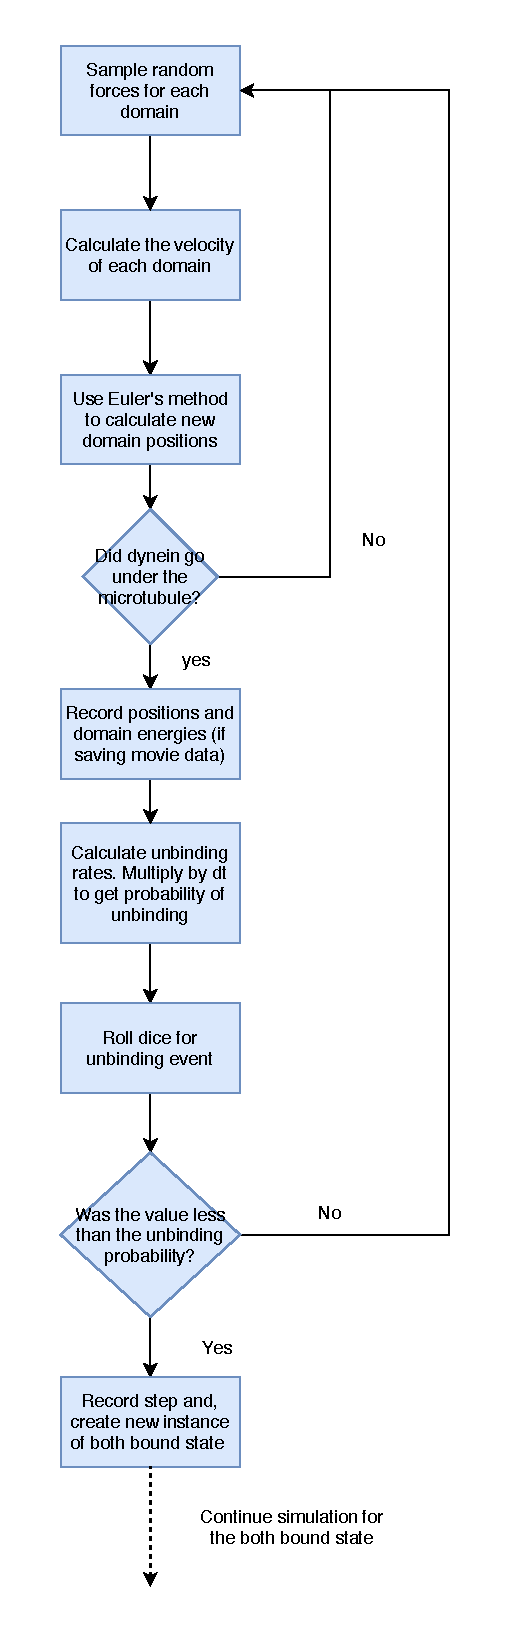
\includegraphics[width=0.39\columnwidth]{One_bound_sim_flowchart.pdf}
		\caption[One bound simulation flow chart]{\textbf{One bound simulation flow chart} showing how the simulation is performed for the one bound state. Note that we do not allow dynein to pass through the microtubule as this is a 2-dimensional simulation.} 
	\end{figure}
	 
	 \newpage
	 
\section{Determining constants of the model}
In order to determine the stalk and tail lengths $\ell_S, \ell_T$, domain radii, and the set of equilibrium angles $\{\varphi_{i,\text{eq}}\}$, we examined microscopy images of dynein in various configurations. The following figure shows a cartoon of the model superimposed on images of real dynein in what we identify as the both bound and one bound states. 
\begin{figure}[hbt!]
	\centering
	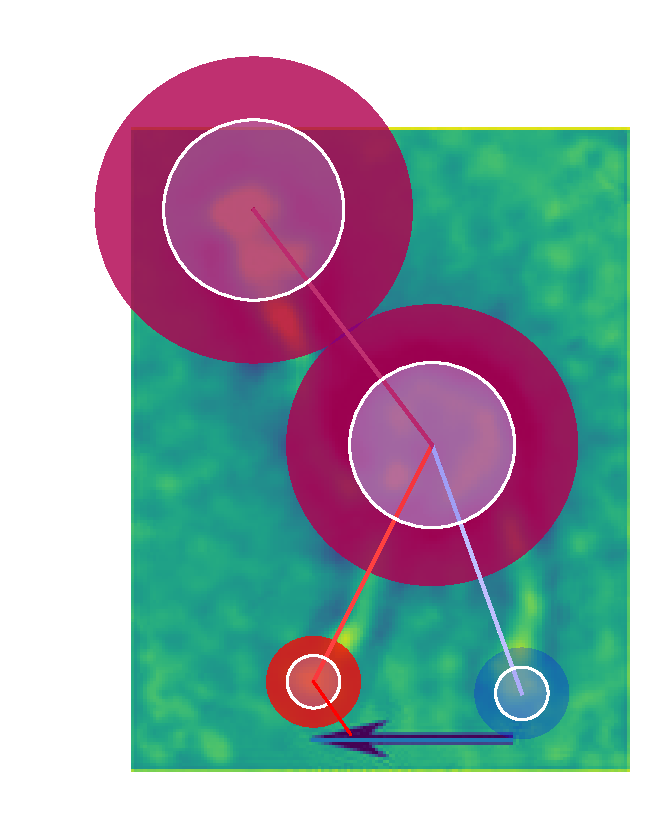
\includegraphics[width=0.3\columnwidth]{burgess-model-figure.pdf}
	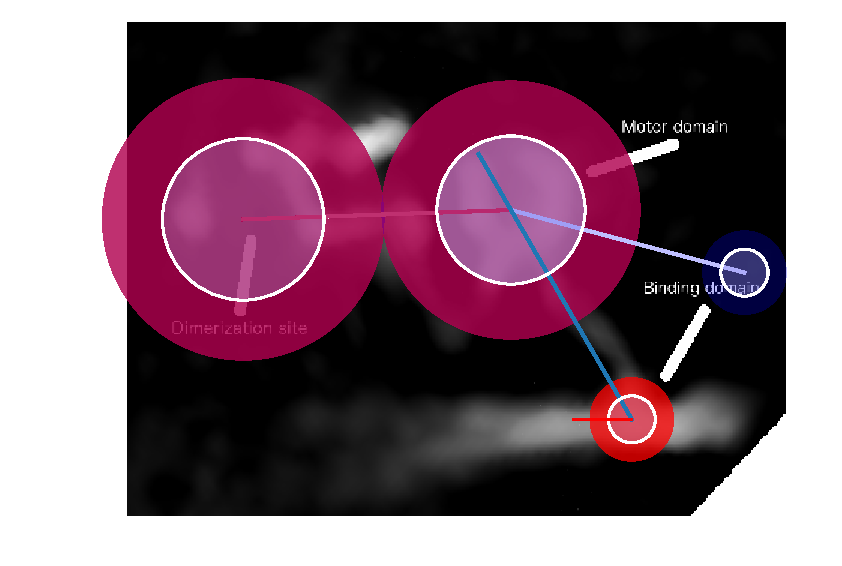
\includegraphics[width=0.5\columnwidth]{grotjahn-model-figure.pdf}%
	\caption[Model parameters determined from experiment ]{\textbf{Model parameters determined from experiment} Left: the both bound model is superimposed over dynein micrograph. The arrow indicates 15nm. Image taken from \cite{burgess2003dynein}.  Right: cryo-electron tomograph of dynein with the one-bound model overlaid. Image taken from \cite{grotjahn}.} 
	\label{fig:superimpmosed}
\end{figure}
Figure \ref{fig:superimpmosed} shows example images of micrographs used to determine the model constants. In order to account for the fact that we idealize the stalks and tail as thin, massless rods, we slightly increase the size of each domain to account for any extra drag. Interestingly, these images suggest an angle of $0^\circ$ for both states.



\section{Testing the model} 
To test the model we ran multiple simulations varying the spring constants and binding / unbinding rates. Having so many degrees of freedom makes using any kind of minimization process challenging to implement and far too long to simulate. Nevertheless, we can still be clever by using reported velocities (for example \cite{dewitt2012cytoplasmic} reports 124 nm/sec) to estimate the time spent in the one bound and both bound states. With this information we can set the binding and unbinding rates in such a way as to simulate only the both bound state \textit{or} the one bound state. With these simulations we can get good estimates for the rate constants. 

With good estimates for these constants, we then refine the values by fitting our stepping statistics to those of experiments such as shown in figures \ref{fig:weihong histogram} and \ref{fig:yildiz_tension}. 
